\chapter{Introduction}

\drop{E}{arth} Observation (\acs{EO}) commercial data sales have increased a 550\% in
the last decade \cite{sousa}[1]. This area is considered a key element in the
space industry and an opportunity market for the next years.

\ac{EO} industries implement on-premises conventional infrastructures to acquire,
store, process and distribute the geo-information generated.

However these solutions have the risks of over/under size the infrastructure, they are not flexible to cover sudden changes in the demand of services and the access to the information presents large latencies.  These aspects limit the use of \ac{EO} technology for real time use such as to manage crises, natural disasters and civil security among others (Deren, 2007).

In addition, new sectors and user typologies are applying for new \ac{EO} services
and there is an increasing demand of this services. These users
need more flexible, easy and instant access to \ac{EO} products and services through
the Web. This demand has traditionally been driven through Space Data
Infrastructures and heavy standards (\acs{ISO} TC/211 and \ac{OGC}) which are focused on
interoperability rather than the real demand from the end-users.

The use of cloud computing technology can overcome the previously defined limitations that present conventional infrastructures because of its elasticity, scalability and on-demand use characteristics (Armbrust, 2010).

GEO-Cloud Experiment goes beyond conventional data infrastructures used in \ac{EO}
industry and beyond the implementations of applications running in cloud, to
quest which parts of a complete infrastructure of \ac{EO} are technologically and
economically viable to be virtualized to offer basic and high added value
services (see Figure~\ref{fig:intr-geocloudConcept}).

\begin{figure}[!h]
\begin{center}
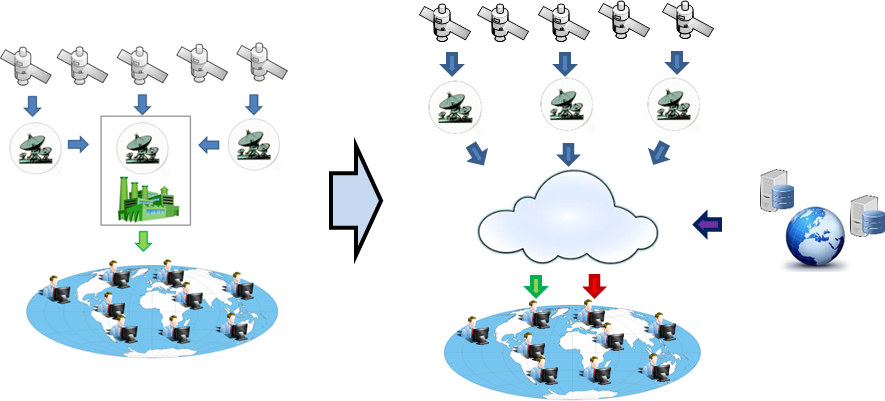
\includegraphics[width=0.7\textwidth]{statement/geocloudConcept.png}
\caption[The GEO-Cloud Concept.]{The GEO-Cloud Concept. It is based on the use of cloud technology to acquire data, store it, process it, integrate it with other sources and distribute it to end users with the final objective of testing viable solutions for its real implementation.}
\label{fig:intr-geocloudConcept}
\end{center}
\end{figure}

GEO-Cloud  emulates the remote sensing mission with the satellites, the
topology network and the communications in the \vw testbed. The data
acquired from the emulated satellites is transferred to the \bonfire cloud
for storage, processing and distribution of data. End users accessing and
broadcasting will be emulated in another network implemented in \vw. In
order to implement realistic impairments in \vw, real networks will be
tested in \pl.  The technologies for imagery distribution and \ac{EO}
service delivery using cloud technologies and Internet protocols will be tested.

\section{Earth Observation}

Since decades, the human's ambitions consists of knowing themselves and
everything outside them. However, technology of that time did not permit these
aims. In last decade, quite technological advances have been carried out and
these goals are the present. Spacecrafts, airplanes, and several technology
elements aggregated by a space mission are designed, built and launched to
retrieve information about the Earth, other planets and galaxies.

The \ac{EO} involves all current technical areas such as Computing, Optics,
Chemistry, Mathematics, Materials, Telecommunications, Aerospace, Physics,
System Engineering among others. The physical, chemical and biological
information about the Earth are gathered using several ways for obtaining the
information and platforms to achieve it.

%https://www.ll.mit.edu/publications/journal/pdf/vol14_no1/14_1activespectral.pdf
%http://nsidc.org/cryosphere/seaice/study/active_remote_sensing.html
%http://earthobservatory.nasa.gov/Features/RemoteSensing/remote_08.php
The Earth surface information can be achieved both actively  and
passively. Active remote sensors as radar emit microwaves toward the Earth's
surface in order to scan objects and areas. These waves reflect off the surface and return to the sensor. This imaging
way is also known as active microwave and three types of actively remote sensing
are: imaging radar, that takes images like a camera depending on the type of
surface where the rays reach; non-imaging radar that measures the amount of reflected energy; and altimetry
sensor which sends microwaves to Earth and measures the time that these
microwaves take to return the sensor.\\
Passive remote sensors use the radiation provided by the objects or surrounding areas. The most common source for gathering passively, is the reflected
sunlight. \\
Passive remote sensors are radiometers for measuring the
electromagnetic radiation, photography to acquire the light reflected by the
chemical elements in visible spectral band, charge-coupled devices catching
ultraviolet spectrum and infrared sensors which obtain thermal images.
Moreover, the \ac{EO} acquisition takes into account three kinds of resolution
for imaging as: the spectral , the geometry and the temporal resolution. The
spectral resolution depends on the object to be sensed. Panchromatic, blue, green , red,
near-infrared and thermal infrared are the
most used spectral bands.

\begin{figure*}
\begin{center}
  \subfloat[Image acquired in blue, near infrared and short wave infrared
  spectral bands.]{
    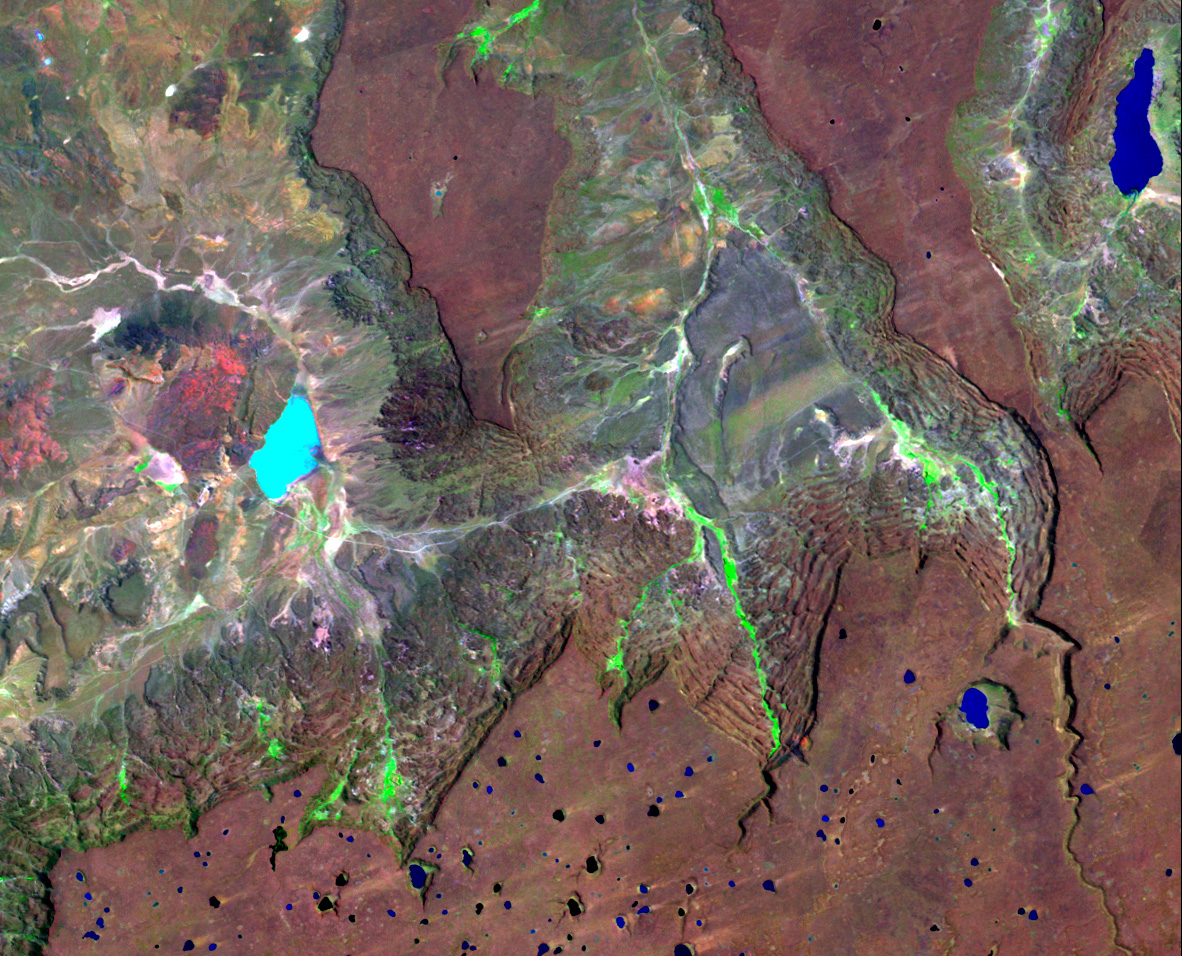
\includegraphics[width=0.4\textwidth]{statement/srtm_l7_basalt.jpg}
    \label{fig:real-view}
  }
 \hspace{0.05\textwidth}
  \subfloat[Image acquired from \ac{SRTM}
  conforming a 3D image.]{
    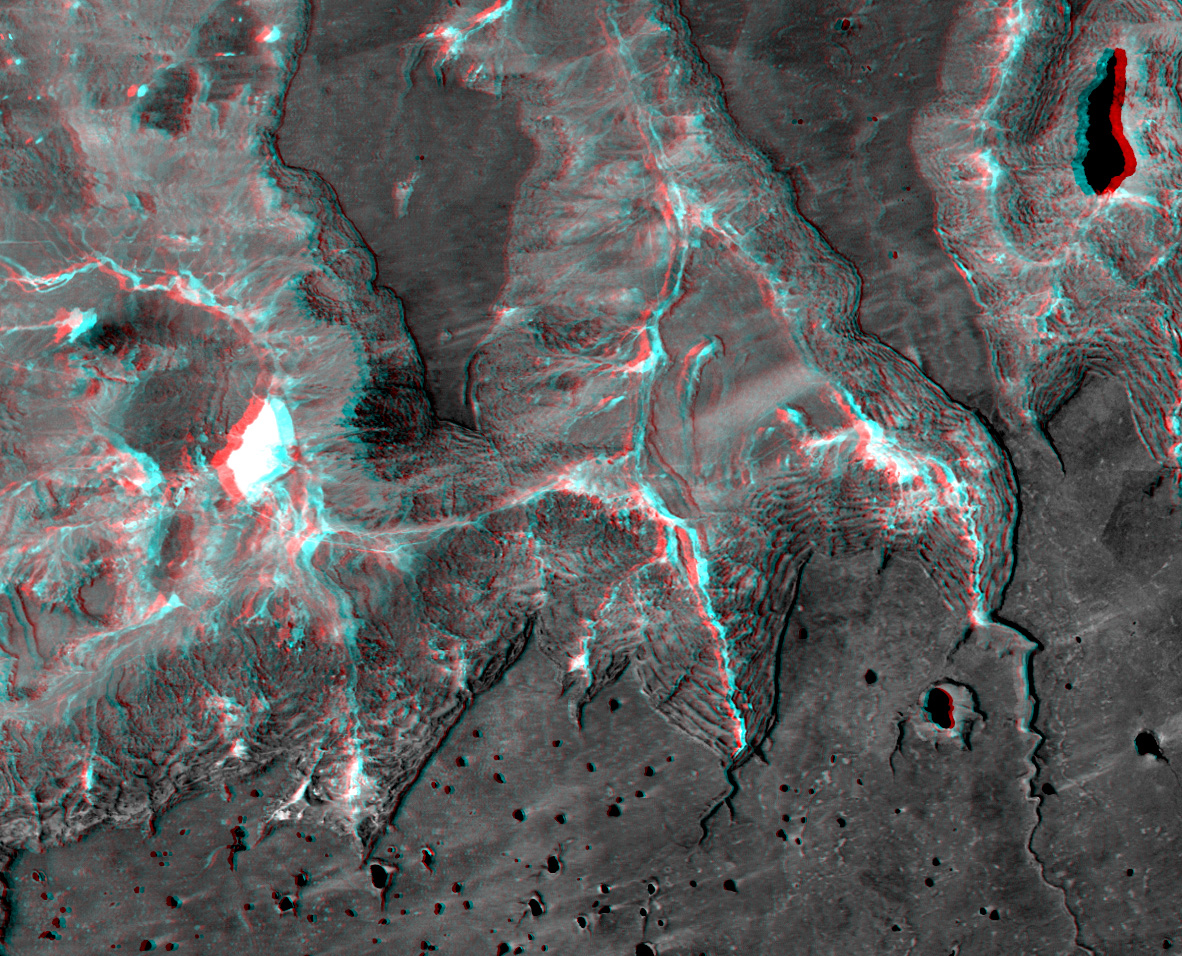
\includegraphics[width=0.4\textwidth]{statement/srtm_anaglyph_basalt.jpg}
    \label{fig:3d-image}
  }
\caption{Different images acquired by \acs{USGS}/\acs{NASA} Landsat.}
\end{center}
\end{figure*}

% \begin{multicols}{2}

% \begin{figure*}
% \begin{center}
% 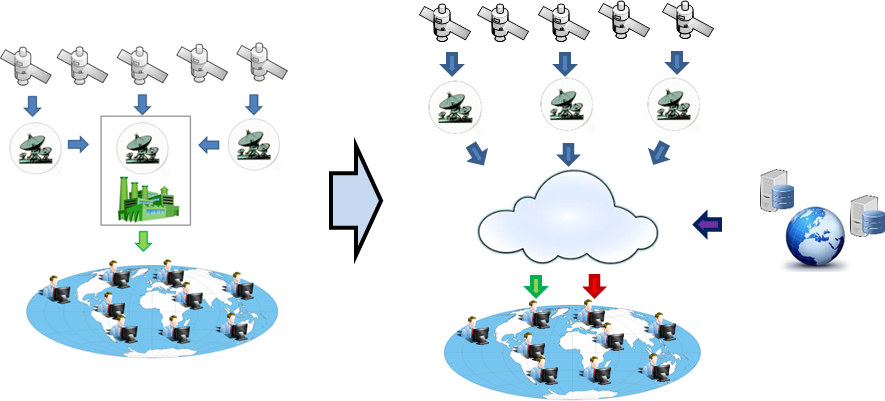
\includegraphics[width=0.2\textwidth]{statement/geocloudConcept.png}
% \caption{The}
% \label{fig:intr-geocloudConcept}
% \end{center}
% \end{figure*}
% \vfill
% \columnbreak
% \begin{figure*}
% \begin{center}
% 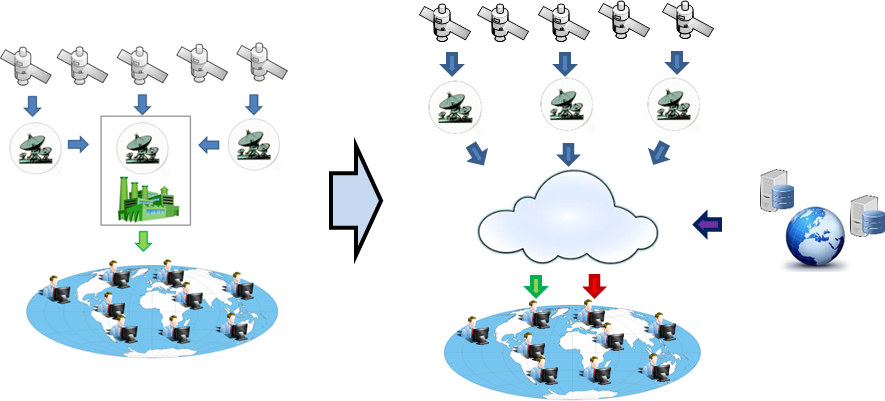
\includegraphics[width=0.2\textwidth]{statement/geocloudConcept.png}
% \caption{The}
% \label{fig:intr-geocloudConcept}
% \end{center}
% \end{figure*}
% \end{multicols}

The geometry resolution is selected depending on how much definition the
telescopes or imaging sensors has to be. If a cloud shall be acquired for
weather applications, the resolution will be about $100km$. In
other hand, if the application is for traffic management, the telescope
resolution must be under $1m$.

The temporal resolution is the frequency between two consecutive
acquisitions of the same location (revisit time). Depending on the image
application, the revisit time can vary. For example, for environmental
monitoring, geology or precision agriculture the revisit time is longer that the
required revisit time for military or maritime surveillance, that
in these cases is critical.

The last component for \ac{EO} imaging consists of the platform where the
payloads for image acquisition are onboard. These platforms are summarized in two sets, spacecrafts and
aircrafts. Aircrafts involve aerodines (planes, and helicopters among
others) and aerostats (balloons and dirigibles). Spacecrafts are systems designed
to fly over the atmosphere and could be used for lots of purposes as communications, \ac{EO},
meteorology and planetary exploration among others.


\section{Cloud Computing}
%http://faculty.winthrop.edu/domanm/csci411/Handouts/NIST.pdf

Traditional business applications have always been too complicated and
expensive. The number and variety of necessary hardware and software to run them
is overwhelming. A team of experts that can install, configure, test, run,
secure, and update is needed.
Thanks to Cloud Computing approach, these
complications do not exist because it is not necessary to manage the hardware
and software: it is the responsibility of an experienced cloud provider. The
shared infrastructure makes it work like a utility: You only pay for what you
need, upgrades are automatic and the enlargement or reduction of the service
comprises a simple process.

The NIST~\ref{NISTrefe} defines \emph{Cloud Computing} as ``Cloud computing is a model for enabling ubiquitous, convenient, on-demand network access to a shared
pool of configurable computing resources (e.g., networks, servers, storage, applications, and services) that
can be rapidly provisioned and released with minimal management effort or
service provider interaction``.

Several cloud deployments are implemented at present. These are:
\begin{itemize}
\item \emph{Private Cloud:} Used by a single organization and it is operated by
  the own organization.
\item \emph{Community Cloud:} Organizations that have shared subjects create
  this kind of cloud in which the managed and support is carried out by the
  organizations themselves.
\item \emph{Public Cloud:} It is provisioned for the general public use it. The
  management of the infrastructure is performed by an academic, business or
  government organization.
\item \emph{Hybrid Cloud:} Cloud composed by distinct infrastructures as public,
  community or private in order to achieve some objectives.
\item \emph{Federated Cloud:} Nowadays, this deployment is growing up
  quickly. The federated architectures are a combination of community, public
  and hybrid clouds in which each one of them offer features that the consumer can
  be used transparently. In the section~\ref{subsec:federatedtools} are detailed.
\end{itemize}

The  cloud computing features are summarized as follows:
\begin{itemize}
\item \emph{On-demand self-service:} A cloud computing user can provision,
  deploy and release computing resources as needed automatically without human
  interaction.
\item \emph{Broad network access:} Cloud capabilities can be accessed by
  standard mechanisms or client platforms.
\item \emph{Resource pooling:} Different resources can be assigned as memory,
  processing capability, network bandwidth among others, and these are
  distributed geographically or into several cloud machines.
\item \emph{Rapid elasticity:} Resources can be elastically provisioned and
  release automatically. This permits to scale rapidly resources.
\item \emph{Measured Service:} Resources can be monitored, controlled and
  reported in order to achieve transparency for the cloud supporter and consumer.
\end{itemize}

The cloud computing infrastructure offers different kinds of services that are
summarized as:

\begin{itemize}
\item \emph{\ac{SaaS}:} The capacity provided to the consumer
  to use   the provider's applications running on the cloud.
\item \emph{\ac{PaaS}:} The capacity provided to the consumer
  consists of the consumer-created applications created by languages, libraries
  and tools supported by the provider can be deployed on the cloud.
\item \emph{\ac{IaaS}:} The capacity provided to the
  consumer consists of provisioning computing resources in order to the consumer
  is able to deploy and run its developed software.
\end{itemize}



\section{The Fed4FIRE European Project}%
%http://www.fed4fire.eu/
The \emph{Fed4FIRE} is an Integrating Project under the European Union's \ac{FP7} which it work programme topic is \emph{Future
  Internet Research and Experimentation}. The project is performed by a
consortium of 29 partner from different countries. The project is coordinated by
the \emph{iMinds}, Belgium.
The \emph{Fed4FIRE} project establishes a common federation framework for
experimenters. A large of number of facilities in Europe are integrated in the
\emph{Fed4FIRE} federation. Such facilities focus on different  areas
of networking. Example domains are wireless networking, cloud computing, smart
cities and grid computing among others.
Also, the \emph{Fed4FIRE} project has to validate its infrastructure to perform
innovative experiments, so researches from different Future Internet areas
are invited. As a result, projects like \emph{GEO-Cloud} are carried out.

\section{The Geo-Cloud Experiment Overview}


\subsection{Experiment Description}

The experiment consists of virtualizing a conventional \ac{EO} system to offer on
demand services to clients with the objective of validating its viability, find
the strengths and weaknesses of using cloud computing technology and establish
possible solutions for a future implementation in the market. There are three
components:
\begin{enumerate}
\item \emph{In-orbit mission:} this component generates the raw data. This consists of un-processed images of the Earth captured by a constellation of satellites and downloaded to different ground stations.
\item \emph{Treatment of data:} the data has to be stored, processed at different levels based on the services offered and distributed to the clients. The data acquired by the in-orbit mission is integrated with other sources to provide higher quality services.
\item \emph{End-users:} users of the provided services with different levels of remote access rights.

\end{enumerate}


\subsubsection{Experiment Design}


The GEO-Cloud experiment requires emulating a complete realistic Earth Observation Mission to provide high added value services such as crisis management. To this complex situation, the system has to response by processing on demand massive and variable amounts of stored and on line transferred data.

GEO-Cloud makes use of the following \emph{Fed4FIRE} facilities: \pl,\vw and
\bonfire. \pl allows us to measure real network characteristics geographically
distributed to setup our models. \vw allows us to create any desired network
topology and emulate the in-orbit mission and the web service to the
users. \bonfire provides us a real cloud infrastructure with observability in
all the layers to test our cloud based services.


\paragraph{Implementation of the acquisition of geo-data in Virtual Wall and
  PlanetLab}~\\
The acquisition of geo-data is obtained from the in-orbit mission. The
constellation of satellites and the ground stations are emulated in \vw. A
network topology is implemented to communicate the different satellites with the ground stations. Every satellite in its orbit and every ground station models are simulated in a node.

The satellite models simulate the orbits and the pass of the satellites over the ground stations. The ground stations models simulate the coverture of the antennas and the download of the data. When a satellite is inside this radius, the satellite downloads the data to the ground station that is visible. The downloaded data in the ground stations is transferred to the \bonfire cloud.

With the \vw network,the \emph{bandwidths, latencies and loss rates} are
controlled.Also a realistic network topology to transfer data between different
nodes is created.

In order to determine the correct link characteristics for the connections
between the ground and the cloud infrastructure, a profiling tool has been
developed for measuring appropriate values for the link impairment between these different geographical locations using the \pl testbed.


\paragraph{Implementation of the cloud based services in BonFIRE}~\\
To facilitate offering the previous services we propose to implement a multi-layered cloud model in the \bonfire cloud infrastructure to generate on demand geo-information. The multi-layered cloud model is constituted of two layers:
\begin{itemize}
\item \emph{Layer 1:} This layer involves the basic satellite imagery services.  It acquires the raw data, stores it, has the first level of processing, distributes the processed data and offers the hosting service.

\item \emph{Layer 2:} This layer involves the high added value services. It can use historical processed, real time captured and pre-processed data from layer 1. This layer processes the information for real time generation of geo-information and offers real time access and distribution to the end-users. Typically, the implementation of high added value EO services involves the ingestion of the raster imagery from the satellites into a spatial database or storage, where it can be refined, simplified, processed or combined with other data sources in vector or raster format. The products, which can be vector or raster data, are distributed or queried using Internet technologies (\ac{OGC} standards like \ac{WMS}) or through Web services (tiles, caches, etcetera).
\end{itemize}

Thus, the whole \ac{EO} system is completely implemented in \emph{Fed4FIRE}, see Figure 3.

\begin{figure}[!h]
\begin{center}
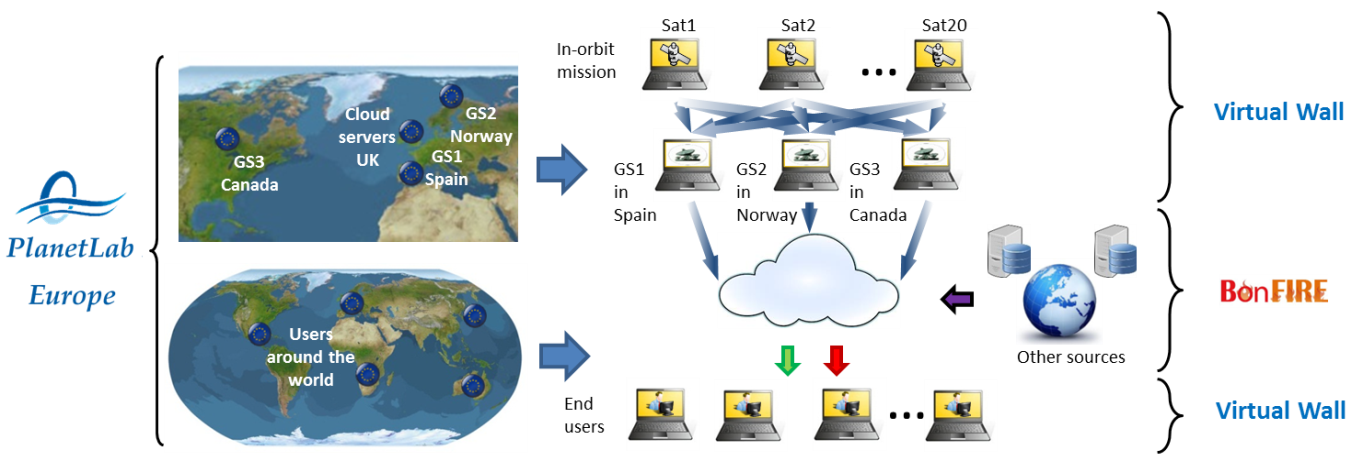
\includegraphics[width=0.7\textwidth]{statement/testbeds-geocloud.png}
\caption{Geo-Cloud implementation in Fed4FIRE}
\label{fig:intr-testbeds-geocloud}
\end{center}
\end{figure}




\subsection{Impact in Fed4FIRE}
The experiment will contribute to several objectives of the \emph{Fed4FIRE} project:
increase trustworthiness of its facilities and support their
sustainability. GEO-Cloud will test \emph{Fed4FIRE} tools for its use in the industry
driven experiments close to market, specifically complex and real time services
for Earth Observation industry when critical situations occur.
GEO-Cloud will validate the tools for monitoring and control of cloud computing
and networking in EO services for emergencies and will test the limits of the
infrastructure for processing, storing and traffic of massive on-demand
data. GEO-Cloud will provide feedback to improve the infrastructure during and
after the experiment is carried out, sharing our knowledge in traditional
infrastructures for \ac{EO} applications, monitoring, processing and
distribution of geospatial data.

\subsection{Scientific and Technological Impact}

GEO-Cloud will contribute to provide a worldwide service in the Earth
Observation Industry. It will answer if Future Internet technologies can provide
viable solutions for the complex \ac{EO} market and to find the limitations of
the current cloud computing technology for its application in \ac{EO} market.

GEO-Cloud will test the viability and ease of use of those facilities for
industry driven experiments close to the market.

\subsection{Socio-Economic Impact}

The Geo-Cloud project is used as a framework to offer services from \ac{EO}
users. The benchmark developed in the experiment allows to establish the
frontiers of viable and not viable cloud solutions in \ac{EO} depending on the
type of demand and service offered. This will establish the basis to satisfy the
growing demand of added value \ac{EO} services.

The reduction of the processing, storage, communications and distribution costs
of \ac{EO} services will facilitate the access to the remote sensing technology of
common end users, but also of a more general public. GEO-Cloud will contribute
defining the basis to advance in the use of geospatial information of the nine
``Societal Benefit Areas'' defined in GEO: disasters, health, energy, climate,
water, weather, ecosystems, agriculture and biodiversity; by demonstrating
whether or not cloud computing offers technologically and economically viable
solutions to offer highly demanding services.

The results obtained in the experiment will be used by our company to offer new
services to the general public, current end users and future potential users. The
rest of the \ac{EO} industry will be beneficiated since we will define a
benchmark that relates the demand with the technology to offer quality
services. The users will be beneficiated since we will define the framework to
offer higher quality services.




\section{Document Structure}

This document has been carried out as the end of carrier project rules from the \emph{Escuela
Superior de Informática} of the \emph{Universidad de Castilla La Mancha}. It contains
the following sections:


\begin{definitionlist}
\item[Chapter \ref{chap:antecedentes}: \nameref{chap:antecedentes}] In this
  chapter an overview of the necessary knowledge areas is made to study for the
  development of GEO-Cloud, like cloud computing, distributed middleware,
  processing premises for \ac{EO} and several testbeds in \emph{Fed4FIRE}.
\item[Chapter \ref{chap:objetivos}: \nameref{chap:objetivos}] In this
  chapter, the main objectives for GEO-Cloud are depicted and explained.
\item[Chapter \ref{chap:method}: \nameref{chap:method}] in this chapter the
  selected methodology is explained and justified. Also, the uses resources such
  \emph{Fed4FIRE's} testbeds, hardware and software are depicted.
\item[Chapter \ref{chap:geocloud-experiment}: \nameref{chap:geocloud-experiment}] In this
  chapter, the entire GEO-Cloud project is explained. The design and implementation of the
  satellite constellation, the design and implementation of the satellites and
  ground stations simulators over \vw, the design and implementation of the
  cloud architecture for \ac{EO} and finally the \pl experiment for acquiring
  network impairments are detailed.
\item[Chapter \ref{chap:evolution}: \nameref{chap:evolution}] In this chapter,
  the project evolution during the development detailing the phases and
  iterations besides the inconveniences and decisions to solve them are
  described. Also, costs of project and schedule are shown.
\item[Chapter \ref{chap:results}: \nameref{chap:results}] In this chapter, the
  results of the development of the project are shown.
\item[Chapter \ref{chap:conclusions}: \nameref{chap:conclusions}]In this
  chapter, the development conclusion and the reached objectives are
  summarized. Some future work and lines of research are suggested.
 \end{definitionlist}
